\newpage
%%%%%%%%%%%%%%%%%%%%%%%%%%%%%%%%%%%%%%%%%%%%%%%%%%%%%%%%%%%%%%%%
%%%%%%%%%%%%%%%%%%%%%%%%%%%%%%%%%%%%%%%%%%%%%%%%%%%%%%%%%%%%%%%%
%%%%%%%%%%%%%%%%%%%%%%%%%% Enunciado %%%%%%%%%%%%%%%%%%%%%%%%%%%

\begin{myblock}
\phantomsection\addcontentsline{toc}{section}{Ejercicio \#4 | Backpropagation}
\section*{Ejercicio \#4 | Backpropagation}

Considera un problema de clasificación multiclase y una red neuronal densamente conectada con una
capa oculta, como se muestra en la figura \ref{fig:red_p02}. Considera también la función Sigmoide como 
activación de las unidades ocultas, la función Softmax para la estimación de las capas finales y
a Cross-Entropy como función de costo. 

\end{myblock}

\begin{figure}[h!]
    \centering
    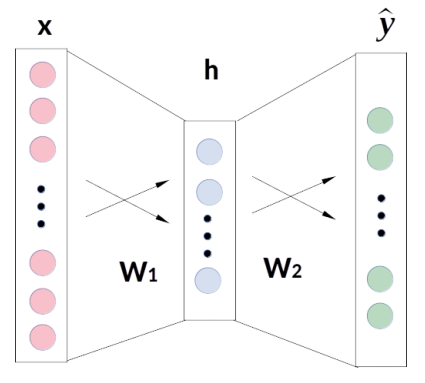
\includegraphics[width=0.4\linewidth]{Images/Red_Problema_02.png}
    \caption{Red neuronal densamente conectada con una sola capa oculta.}
    \label{fig:red_p02}
\end{figure}

%%%%%%%%%%%%%%%%%%%%%%%%%%%%%%%%%%%%%%%%%%%%%%%%%%%%%%%%%%%%%%%%
%%%%%%%%%%%%%%%%%%%%%%%%%%%%%%%%%%%%%%%%%%%%%%%%%%%%%%%%%%%%%%%%

%%%%%%%%%%%%%%%%%%%%%%%%%%%%%%%%%%%%%%%%%%%%%%%%%%%%%%%%%%%%%%%%
%%%%%%%%%%%%%%%%%%%%%%%%%%%%%%%%%%%%%%%%%%%%%%%%%%%%%%%%%%%%%%%%


\subsection{Teoría}


%%%%%%%%%%%%%%%%%%%%%%%%%%%%%%%%%%%%%%%%%%%%%%%%%%%%%%%%%%%%%%%%
%%%%%%%%%%%%%%%%%%%%%%%%%%%%%%%%%%%%%%%%%%%%%%%%%%%%%%%%%%%%%%%%

\begin{myblock}
    
    \textbf{(a)} Muestra que Softmax es invariante a traslaciones constantes del vector de entrada
    i.e. para cualquier vector $x$ y cualquier constante $C$:

    \[
        \text{Softmax}(x) = \text{Softmax}(x + c)
    \]

    Donde la operación $x+c$ se realiza con broadcasting. Recuerda que:

    \[
        \text{Softmax}(x) = \frac{e^{x_i}}{\sum_{j} e^{x_j}}
    \]

    Lo anterior es útil cuando se escoge $c = -\text{max}(x)$ i.e. quitando el valor mayor
    en todos los elementos de $x$ para mejorar la estabilidad numérica. 
\end{myblock}

Para resolver este inciso, conviene primero recordar lo que es broadcasting. Este mecanismo
nos permite operar arreglos de forma que se puede replicar, si hacer copias en memoria, un 
arreglo de menor dimensión a uno de mayor dimensión. Para el caso de $x \in \mathbb{R}^d$ ya
un escalar $c \in \mathbb{R}$, la operación $x+c$ consistiría en replicar ese $c$ a lo largo 
de toda la coordenada de $x$, tal que:

\[
    x+c = (x_1 + c, x_2 + c,..., x_d + c)
\]  

Recordemos también la definición de la función Softmax:

\[
    \text{Softmax}(x)_i = \frac{e^{x_i}}{\sum_{j=1}^{k} e^{x_j}} \;\;\;\;\;\; \text{con} \;\; i = 1,2,...,d 
\]

De ese modo, si consideramos al vector $x+c$ trasladado, entonces nos encontraremos con:

\[
    \boxed{\text{Softmax}(x+c)_i = \frac{e^{x_i + c}}{\sum_{j=1}^{k} e^{x_j + c}} = \frac{e^c \cdot e^{x_i}}{e^c \cdot \sum_{j=1}^{k} e^{x_j}} = \frac{e^{x_i}}{\sum_{j=1}^{k} e^{x_j}}  = \text{Softmax}(x)_i}
\]

Esta demostración nos está diciendo que, bajo las condiciones que establecimos, Softmax
solo depende de las diferencias entre los componentes en $x$, no de sus valores absolutos.
En otras palabras, podemos decir que el mecanismo de broadcasting permite escribir al vector
$x+c$ como $x+c = (x_1, x_2,...,x_d)+c$. 

Además, se evitan valores muy grandes que se cargarían por la operación suma entre cada entrada 
del vector $x$ con la constante $c$, algo que podría causar problemas de desbordamiento en el 
cómputo de la memoria. 

\begin{myblock}
    \textbf{(b)} Para un escalar $x$, muestra que el gradiente de la función Sigmoide es: 

    \[
        \sigma(x) = (1 - \sigma(x))
    \]
\end{myblock}

Nosotros ya sabemos que la Sigmoide se define como:

\[
    \sigma(x) = \frac{1}{1 - e^{-x}}
\]

Entonces, si derivamos utilizando regla de la cadena, tenemos:

\begin{align*}
        \sigma'(x) &= \frac{d}{dx} \big[(1 - e^{-x})^{-1}\big] = (-1) (1 - e^{-x})^{-1-1} \cdot (-e^{-x})\\
                   &= -(1 - e^{-x})^{-2} \cdot (-e^{-x}) \\
                   &= \frac{e^{-x}}{(1-e^{-x})^2} 
\end{align*}

Ahora, bien:

\[
    1 - \sigma(x) = 1 - \frac{1}{1 - e^{-x}} = \frac{1 - (1- e^{-x})}{1 - e^{-x}} = \frac{e^{-x}}{1 - e^{-x}}
\]

Por lo tanto: 

\[
    \boxed{\sigma(x) \cdot (1 - \sigma(x)) = \frac{1}{1 - e^{-x}} \cdot \frac{e^{-x}}{1 - e^{-x}} = \frac{e^{-x}}{(1 - e^{-x})^2} = \sigma'(x)}
\]

Lo que todo este desarrollo nos está diciendo es que podemos obtener la derivada de la sigmoide sin necesidad de clacular
directamente con la regla de la cadena. Es decir, podemos definirla solo como el producto de la misma 
Sigmoide con ella misma. La primer conclusión que podríamos pensar respecto a este resultado es que ahorramos
poder computacional durante el Backpropagation, así como ahorro en la memoria, ya que se utilizan resultados previos,
haciendo que el algorito de retropropagación sea más eficiente. Es una construcción de la derivada de la 
Sigmoide que facilita la propagación del error hacia las capas ocultas. 

%%%%%%%%%%%%%%%%%%%%%%%%%%%%%%%%%%%%%%%%%%%%%%%%%%%%%%%%%%%%%%%%
%%%%%%%%%%%%%%%%%%%%%%%%%%%%%%%%%%%%%%%%%%%%%%%%%%%%%%%%%%%%%%%%

\begin{myblock}
    
    \textbf{(c)} Muestra que el gradiente de la capa de salida es:

    \[
        \frac{\partial L(y, \hat{y})}{\partial z} = \hat{y} - y
    \]

    Donde $\hat{y} = \text{Softmax}(z)$ para algún vector $z$ que proviene de la capa de salida. Qué interpretación
    puedes darle a esa expresión? LA función de costo es Cross-Entropy:

    \[
        L(y, \hat{y}) = - \sum_i y_i \log(\hat{y})
    \]

    Aquí $y$ es un vector \textit{one-hot} de las clases y $\hat{y}$ de las probabilidades estimadas. 
\end{myblock}

Sean los logits $z \in \mathbb{R}^d$, ya sabemos que Softmax se define como:

\[
    \hat{y}_i = \frac{e^{x_i}}{\sum_{j} e^{x_j}}
\]

Y que la pérdida es una Cross-Entropy:

\[
    L(y, \hat{y}) = - \sum_i y_i \log(\hat{y})
\]

Ahora, como estamos trabajando con una $y$ en \textit{one-hot encoding}, tenemos que:

\[
    \frac{\partial L}{\partial z_j} = \frac{\partial L}{\partial \hat{y}_i} \frac{\partial \hat{y}_i}{\partial z_j}
\]

Tenemos que:

\[
    \frac{\partial L}{\partial \hat{y}_i} = -\frac{y}{y_i} y \;\;\;\;\; => \;\;\;\;\; \frac{\partial \hat{y}_i}{\partial z_i} = \hat{y} (\delta_{ij} - \hat{y}_j)
\]

En este caso, estamos usnado la delta de Kronecker, definida como:

\[
    \delta_{ij} = \begin{cases}
         1 & \text{si} \;\; i=j\\
         0 & \text{si} \;\; i \neq j
    \end{cases}
\]


La probabilidad de la clase $i$ se define como:
\[
\hat{y}_i = \frac{e^{z_i}}{\sum_k e^{z_k}}
\]
Aplicamos la regla del cociente para derivar con respecto a $z_i$:
\[
\frac{\partial \hat{y}_i}{\partial z_i} = \frac{ \left(\frac{\partial}{\partial z_i}e^{z_i}\right) \left(\sum_k e^{z_k}\right) - e^{z_i} \left(\frac{\partial}{\partial z_i}\sum_k e^{z_k}\right) }{\left(\sum_k e^{z_k}\right)^2}
\]
\[
= \frac{ e^{z_i} \left(\sum_k e^{z_k}\right) - e^{z_i} (e^{z_i}) }{\left(\sum_k e^{z_k}\right)^2}
\]
Separando la fracción:
\[
= \frac{e^{z_i}}{\sum_k e^{z_k}} - \frac{e^{z_i}e^{z_i}}{\left(\sum_k e^{z_k}\right)^2}
\]
\[
= \frac{e^{z_i}}{\sum_k e^{z_k}} \left(1 - \frac{e^{z_i}}{\sum_k e^{z_k}}\right)
\]
Lo que simplifica a:
\[
= \hat{y}_i(1 - \hat{y}_i)
\]

Ahora, derivamos $\hat{y}_i$ con respecto a una entrada diferente, $z_j$. La variable $z_j$ solo aparece en el denominador.
\[
\frac{\partial \hat{y}_i}{\partial z_j} = \frac{ \left(\frac{\partial}{\partial z_j}e^{z_i}\right) \left(\sum_k e^{z_k}\right) - e^{z_i} \left(\frac{\partial}{\partial z_j}\sum_k e^{z_k}\right) }{\left(\sum_k e^{z_k}\right)^2}
\]
Como $i \neq j$, la derivada del numerador es cero:
\[
= \frac{ 0 \cdot \left(\sum_k e^{z_k}\right) - e^{z_i} (e^{z_j}) }{\left(\sum_k e^{z_k}\right)^2}
\]
\[
= - \frac{e^{z_i} e^{z_j}}{\left(\sum_k e^{z_k}\right)^2}
\]
Reagrupando los términos:
\[
= - \left(\frac{e^{z_i}}{\sum_k e^{z_k}}\right) \left(\frac{e^{z_j}}{\sum_k e^{z_k}}\right)
\]
Lo que simplifica a:
\[
= -\hat{y}_i \hat{y}_j
\]

Podemos escribir ambos casos en una sola expresión usando el delta de Kronecker, $\delta_{ij}$:
\[
\frac{\partial \hat{y}_i}{\partial z_j} = \hat{y}_i(\delta_{ij} - \hat{y}_j)
\]
Donde $\delta_{ij}$ es 1 si $i=j$ y 0 en caso contrario.

\paragraph*{Si $i=j$:}
$\delta_{ij}=1$, entonces la expresión se convierte en:
\[
\frac{\partial \hat{y}_i}{\partial z_j} = \hat{y}_i(1 - \hat{y}_j)
\]

\paragraph*{Si $i \neq j$:}
$\delta_{ij}=0$, entonces la expresión se convierte en:
\[
\frac{\partial \hat{y}_i}{\partial z_j} = \hat{y}_i(0 - \hat{y}_j) = -\hat{y}_i \hat{y}_j
\]

Entonces:

\[
    \frac{\partial L}{\partial z_j} = \sum_{i} \big(- \frac{y_i}{\hat{y}_i}\big) \hat{y_i} \big(\delta_{ij} - \hat{y}\big) = \sum_{i} \big(-y_i (\delta_{ij} - \hat{y}_i)\big) = -y_j + \hat{y}_j \sum_{i} y_i
\]

Como tenemos $y$ en \textit{one-hot}, tenemos que $\sum_{i} y_i = 1$:

\[
    \frac{\partial L}{\partial z_j} = \hat{y}_j - y_j \;\;\;\;\; => \;\;\;\;\; \nabla_z L = \hat{y} - y
\]


De todo lo anterior, podemos observar que Softmax convierte logits en probabilidades, Cross-Entropy penaliza
desviaciones respecto a $y$ y que el gradiente $\hat{y} - y$ indica cuánto tenemos de probabilidad por clase. 


%%%%%%%%%%%%%%%%%%%%%%%%%%%%%%%%%%%%%%%%%%%%%%%%%%%%%%%%%%%%%%%%
%%%%%%%%%%%%%%%%%%%%%%%%%%%%%%%%%%%%%%%%%%%%%%%%%%%%%%%%%%%%%%%%

\begin{myblock}
    
    \textbf{(d)} Considerando los incisos anteriores, obtén los gradientes respecto a los parámetros del
    modelo calculando:

    \[
        \bigg\{\frac{\partial (y, \hat{y})}{\partial x} \bigg\}
    \]

    Para, de esa manera, obtener las ecuaciones de Backpropagation de la red. Recuerda que el paso Forward
    calcula las activaciones:

    \[
        h = \sigma(w_1 x + b_1)
    \]

    \[
        \hat{y} = \text{Softmax}(w_2 h + b_2)
    \]

    Recordemos también que la función de activación en un vector se aplica entrada por entrada. 
\end{myblock}


Creo que es buena idea comenzar hablando un poco sobre el proceso de retropropagación y cómo es tan
fundamental para el desarrollo de las Redes Neuronales. Backpropagation consiste en la optimización
iterativa de los parámetros internos de la red neuronal, i.e. los pesos y los sesgos. Lo que se busca
es minimizar la función de pérdida que se encarga de cuantificar el error de las predicciones y los
valores verdaderos. Este mecanismo se trata entonces de un algoritmo fundamental que permite el proceso
de aprendizaje, claculando de manera efiicente el gradiente de la función de pérdida con respecto a cada
parámetro de la red. Intentaremos desglozar el proceso. 

Ya sabemos que el Forward Pass es el proceso en el cual la red transforma una entrada $x$ en una
predicción $y$. Cada entrada $x$ se procesa en una transformación lineal utilizando la matriz de pesos
$W_1$ y el vector de sesgos $b_1$ de la capa de entrada. A este resultado se le suele llamar ``vector de
preactivaciones'', $a_n$. 

\[
    a_1 = W_1 x + b_1
\]

Al vector de preactivaciones se le pasa hacia una función de activación no lienal, en nuestro caso una
Sigmoide.

\[
    h = \sigma(a_1)
\]

Las activaciones $h$ de la capa oculta son procesadas por una segunda transformación lineal, utilizando 
ahora los parámetros $W_2$ y $b_2$, para generar así un vector de puntuaciones $z$:

\[
    z = W_2 h + b_2
\]

Finalmente, el vector $z$ se le normaliza mediante una Softmax, que lo transforma en una distribución de 
probabilidad multinomial, $\hat{y}$, donde cada elemento representea la probabilidad predicha por cada clase:

\[
    \hat{y} = \text{Softmax}(z)
\]

Ahora bien, la cuantificación de la pérdida. Sabemos que la discrepancia entre la predicción $\hat{y}$ y la 
etiqueta $y$, en \textit{one-hot}, se cuantifica mediante la función de pérdida Cross-Entropy categórica $L$. 
Esta función mide la divergencia de información entre las dos distribuciones:

\[
    L = -\sum_{i} y_i \log (\hat{y})
\]

El objetivo del aprendizaje es, entonces, minimizar el valor de $L$ a través del ajuste de los parámetros:

\[
    \theta = \{W_1,b_1, ..., W_n, b_n\}
\]

El cálculo de los gradientes de la función de pérdida $L$ con respecto a los parámetros $W_2$ y $b_2$ de la
capa de salidad mediante la aplicación de la regla de cadena. PArtimos de la expresión conocida de la derivada
de la pérdiad con respecto al vector de puntuaciones $z$:

\[
    \delta = \frac{\partial L}{\partial z} = \hat{y} - y
\]

Aquí, $\hat{y}$ es el vector de probabilidades predichas y $y$ es el vector de etiquetas reales. Así, definimos
$z$ como: $z = W_2 h + b_2$ con $h$ como el vector de observaciones de la capa oculta con dimensión $H \times 1$
y $W_2$ con dimensiones $C \times H$. En este caso, tenemos $C$ como la dimensión de las clases y $H$ como la 
dimensión o cantidad de neuronas por capa oculta. Entonces:

\[
    \frac{\partial L}{\partial W_2} = \frac{\partial L}{\partial z} \cdot \frac{\partial z}{\partial W_2}
\]

Dado que $\frac{\partial L}{\partial z} = \delta$, hay que concentrarse en $\frac{\partial z}{\partial W_2}$. 
Calculamos la derivada de $L$ con respecto a cada elemento de $W_{2ij}$ de $W_2$:

\[
    z_i = \sum_{H}^{k = 1} W_{2ik} h_k + b_{2i}
\]

\[
    \frac{\partial z_i}{\partial W_{2ij}} = h_j \;\;\;\;\; \text{para} \;\; k \neq j \;\;\;\;\; \frac{\partial z_i}{\partial W_{2ij}} = 0
\]

\[
    \frac{\partial L}{\partial W_{2ij}} = \sum_{k = 1}^{C} \frac{\partial L}{\partial z_k} \cdot \frac{\partial z_k}{\partial W_{2ij}} = \delta h^\top
\]

Por lo tanto:

\[
    \frac{\partial L}{\partial W_2} = \delta h^\top
\]

Calculando de una manera similar a $\frac{\partial L}{\partial b_2}$:

\[
    \frac{\partial L}{\partial b_2} = \frac{\partial L}{\partial z} \cdot \frac{\partial z}{\partial b_2}
\]

Entonces, para cada elemento $b_{2i}$ de $b_2$, tenemos:

\[
    \frac{\partial z_i}{\partial b_{2i}} = 1
\]

Y para cada $k \neq i$ tenemos:

\[
    \frac{\partial z_i}{\partial b_{2i}} = 0 \;\;\;\;\; \text{entonces} \;\; \frac{\partial z_i}{\partial b_{2i}} = \sum_{k=1}^{C} \frac{\partial L}{\partial z_{k}} \frac{\partial z_k}{\partial b_{2i} = \frac{\partial L}{\partial z_{i}}} \cdot 1 = \delta
\]

Por lo tanto:

\[
    \frac{\partial L}{\partial b_{2}} = \delta = \hat{y} - y
\]

Los gradientes de la pérdida $L$ con respecto a los parámmetros de la capa de salida son:

\[
    \boxed{\frac{\partial L}{\partial W_{2}} = \delta h^\top \;\;\;\;\;\;\; \frac{\partial L}{\partial b_{2}} = \delta}
\]

Estos resultados muestran cómo el error en $delta$ se propaga hacia atrás, a través de la red, utilizando
laas activaciones $h$ de la capa oculta para ajustar los pesos $W_2$ y directamente asignando el error a los 
sesgos $b_2$. 

Una vez calculados los graidentes de la salida, se procede a propagar el error hacia la capa oculta. 
Este proceso implica calcular el gradiente de la pérdiad $L$ con respecto a las activaciones $a_1$
de la capa oculta, denotando como $\delta^h = \frac{\partial L}{\partial a_1}$, y luego utilizar este
valor para obtener los gradientes de los parámetros $W_1$ y $b_1$. 

Las activaciones $h$ se obtienen aplicando la Sigmoide de las preactivaciones $a_1$, i.e. $h = \sigma(a_1)$.
Para encontrar $\delta^h$, usamos regla de la cadena:

\[
    \delta^h = \frac{L}{\partial a_1} = \frac{\partial L}{\partial h} \cdot \frac{\partial L}{\partial a_1}
\]

La derivación de la Sigmoide es $\sigma'(a_1) = \sigma(a_1)(1 - \sigma(a_1)) = h \odot (1 - h)$. Aquí
$\odot$ se define como el producto de Hadamard, i.e. elemento a elemento. 

Dado que $h$ es un vector, $\frac{\partial h}{\partial a_1}$ es una matriz diagonal cn elementos $h_i(1 - h_i)$.
Al multiplicar por el vector $\frac{L}{\partial h}$, esto equivale a un producto elemento a elemento:

\[
    \delta^h = \frac{\partial L}{\partial h} \odot \sigma'(a_1) = \big(W_2^\top \delta\big) \odot \big(h \odot (1- h)\big)
\]

En este caso, $\delta^h$ es de dimensión $H \times 1$, y se trata del error propagado hacia las preactivaciones
de la capa. 

Ahora bien, el cálculo de los gradientes de los parámetros de la capa de entrada con $W_1$ y $b_1$. 

Tenemos $\delta^h = \frac{\partial L}{\partial a_1}$. Calculamos los gradientes para $W_1$ y $b_1$. Las preactivaciones
se definen como: $a_1 = W_1 x + b_1$. Entonces:

\[
    \frac{\partial L}{\partial W_1} = \frac{\partial L}{\partial a_1} \cdot \frac{\partial a_1}{\partial W_1} = \delta^h \frac{\partial a_1}{\partial W_1} = \delta^h x^\top
\]

Así:

\[
    \frac{\partial L}{\partial b_1} = \frac{\partial L}{\partial a_1} \cdot \frac{\partial a_1}{\partial b_1} = \delta^h
\]

Así, Backpropagation se encarga de mover el error hacia atrás de la salida. Este mecanismo es esencial apra el ajuste
iterativo de los pesos y sesgos del modelo, intentando mejorar tras cada época los valores para obtener una mejorar
predicción en la salida.  

%%%%%%%%%%%%%%%%%%%%%%%%%%%%%%%%%%%%%%%%%%%%%%%%%%%%%%%%%%%%%%%%
%%%%%%%%%%%%%%%%%%%%%%%%%%%%%%%%%%%%%%%%%%%%%%%%%%%%%%%%%%%%%%%%




\subsection{Resumen de código}

\subsection{Resultados}

\subsection{Conclusiones}

\clearpage